\documentclass[12pt]{report}
\usepackage[utf8]{inputenc}
\usepackage{amsmath,amssymb,amsthm,enumitem,fourier, empheq}
\usepackage{subfiles}
\usepackage{geometry}
\usepackage[titlenotnumbered,ruled,vlined]{algorithm2e}
\usepackage{mathtools}

\geometry{a4paper, left=20mm, right=20mm, top=20mm, bottom=20mm}

\newcommand{\Z}{\mathbb{Z}}

\theoremstyle{definition}
\newtheorem*{exer}{Exercise}

\DeclarePairedDelimiter{\nint}\lfloor\rceil
\DeclareMathOperator*{\Vol}{Vol}

\title{An Introduction to Mathematical Cryptography \\ \textit{Solutions}}
\author{Le Quoc Dung}
\date{\today}

\begin{document}

\begin{titlepage}
   \begin{center}
        \vspace*{1cm}
        \huge
        \textbf{An Introduction to Mathematical Cryptography}

        \vspace{0.5cm}
        \textit{Solutions}
            
        \vspace{1.5cm}
        \large 
         Solutions for \textit{An Introduction to Mathematical Cryptography (2014) - Hoffstein, Pipher, Silverman} 
            
        \vspace{0.8cm}
        
        \textbf{Le Quoc Dung}
        
        \vspace{1cm}
        
        \vfill
        
        Moscow
            
   \end{center}
\end{titlepage}

\chapter*{Chapter 2}
\begin{exer}[2.3]
Let $g$ be a primitive root of $\mathbb{F}_p$

\begin{enumerate}
    \item[(a)] Suppose that $x = a$ and $x = b$ are both integer solutions to the congruence $g^x \equiv h$ (mod $p$). Prove that $a \equiv b$ (mod $p-1$). Explain why this implies that the map (2.1) on page 64 is well-defined
    \item[(b)] Prove that $\log_g(h_1 h_2) = \log_g(h_1) + \log_g(h_2)$ for all $h_1, h_2 \in \F^*_p$
    \item[(c)] Prove that $\log_g(h^n) = n\log_g(h)$ for all $h \in \mathbb{F}^{*}_p$ and $n \in \mathbb{Z}$
\end{enumerate}
\end{exer}

\begin{proof}
\begin{enumerate}[itemsep=0pt]
    \item [(a)] Because $a$ and $b$ are both solutions to the congruence $g^x \equiv h$ (mod $p$),

    \begin{equation*}
        \begin{cases}
        g^a \equiv h \quad (\text{mod}\ p) \\
        g^b \equiv h \quad (\text{mod}\ p)
        \end{cases}
    \end{equation*}


    $\Rightarrow$ $g^{-b} \equiv h^{-1}$ (mod $p$)
    
    $\Rightarrow$ $g^ag^{-b} \equiv hh^{-1} \equiv 1$ (mod $p$)
    
    $\Rightarrow$ $g^{a-b} \equiv 1$ (mod $p$), but $g$ is primitive root of $\mathbb{F}_p$
    
    $\Rightarrow$ $\phi(p) | (a-b)$ $\Leftrightarrow$ $(p-1) | (a-b)$
    
    $\Rightarrow$ $a - b \equiv 0$ (mod $p-1$)
    
    $\Rightarrow$ $a \equiv b$ (mod $p-1$)

    \item[(b)] Suppose that 
    
    \begin{equation*}
        \begin{cases}
        h_1 \equiv g^{x_1} \quad (\text{mod}\ p) \\
        h_2 \equiv g^{x_2} \quad (\text{mod}\ p)
        \end{cases}
    \end{equation*}
    
    $\Rightarrow$ $x_1=\log_g h_1$ and $x_2=\log_g h_2$ (1)
    
    And $h_1 h_2 \equiv g^{x_1 + x_2}$ (mod $p$)
    
    $\Rightarrow$ $x_1 + x_2 = \log_g(h_1 h_2)$ (2)
    
    From (1) and (2), $\log_g h_1 + \log_g h_2 = \log_g (h_1 h_2)$
    
    \item[(c)] Same as (b).
\end{enumerate}

\end{proof}

\begin{exer}[2.5]
Let $p$ be an odd prime and let $g$ be a primitive root modulo $p$. Prove that $a$ has a square root modulo $p$ if and only if its discrete logarithm $\log_g(a)$ modulo $p-1$ is even. 
\end{exer}

We have $g^{p-1} \equiv 1$ (mod $p$).

\begin{enumerate}
    \item [(1)] If $a$ has square root modulo $p$, then there is $b$: $b \equiv a^2$ (mod $p$)
    
    $\Rightarrow \log_ga = \log_g(b^2) = 2\log_gb$ (mod $p-1$)
    
    $\Rightarrow$ $\log_ga$ is even. 
    
    \item [(2)] If $\log_ga$ modulo $p-1$ is even
    
    $\Rightarrow \log_ga = 2\log_gb$ (mod $p-1$) with some $b \in \F_p$
    
    $\Rightarrow \log_ga = \log_g(b^2)$ (mod $p-1$)
    
    $\Rightarrow a \equiv b^2$ (mod $p-1$)
    
    $\Rightarrow$ $a$ has square root modulo $p-1$
\end{enumerate}

\begin{exer}[2.10]
The exercise describes a public key cryptosystem that requires Bob and Alice to exchange several messages. We illustrate the system with an example.

Bob and Alice fix a publicly known prime $p=32611$, and all of other numbers used are private. Alice takes her message $m=11111$, chooses a random exponent $a=3589$, and sends the number $u=m^a$ (mod $p$) $=15950$ to Bob. Bob chooses a random exponent $b=4037$ and sends $v=u^b$ (mod $p$) $=15422$ back to Alice. Alice then computes $w=v^{15619} \equiv 27257$ (mod $32611$) and sends $w=27257$ to Bob. Finally, Bob computes $w^{31883}$ (mod $32611$) and recovers the value $11111$ of Alice's message.

\begin{enumerate}
    \item [(a)] Explain why this algorithm works. In particular, Alice uses the numbers $a=3589$ and 15619 as exponents. How are they related? Similarly, how are Bob's exponents $b=4037$ and 31883 related?
    \item [(b)] Formulate a general version of this cryptosystem, i.e., using variables, and show how it works in general.
    \item [(c)] What is the disadvantage of this cryptosystem over Elgamal? (\textit{Hint.} How many times must Alice and Bob exchange data?)
    \item [(d)] Are there any advantages of this cryptosystem over Elgamal? In particular, can Eve break it if she can solve the discrete logarithm problem? Can Eve break it if she can solve the Diffie-Hellman problem?
\end{enumerate}
\end{exer}

\begin{proof}

(a) We have $3589x15619 \equiv 4073x31883 \equiv 1$ (mod $p-1$)

(b) Alice chooses $a$ and $a'$ satisfy that $aa' \equiv 1$ (mod $p-1$)

Bob chooses $b$ and $b'$ satisfy that $bb' \equiv 1$ (mod $p-1$)

From this, we have $aa' = k(p-1)+1$ and $bb' = l(p-1) + 1$

$\Rightarrow v \equiv u^b \equiv (m^a)^b \equiv m^{ab}$ (mod $p$)

$\Rightarrow w \equiv v^{a'} \equiv (m^{ab})^{a'} \equiv m^{aa'b}$ (mod $p$)

$\Rightarrow w^{b'} \equiv m^{aa'bb'} \equiv m^{[k(p-1)+1]x[l(p-1)+1]} \equiv m^{D(p-1)+1} \equiv m$ (mod $p$)
\end{proof}

\begin{exer}[2.11]
The group $S_3$ consists of the following six distinct elements

\begin{center}
    $e$, $\sigma$, $\sigma^2$, $\tau$, $\sigma\tau$, $\sigma^2\tau$
\end{center}

where e is the identity element and multiplication is performed using the rules

\begin{center}
    $\sigma^3 = e$, \quad $\tau^2 = e$, \quad $\tau\sigma = \sigma^2\tau$
\end{center}

Compute the following values in the group $S_3$:

(a)  $\tau\sigma^2$ \quad\quad (b)  $\tau(\sigma\tau)$ \quad\quad (c)  $(\sigma\tau)(\sigma\tau)$ \quad\quad (d)  $(\sigma\tau)(\sigma^2\tau)$

Is $S_3$ a commutative group?
\end{exer}

\begin{proof}
(a) $\tau\sigma^2 = \tau\sigma\sigma = \sigma^2\tau\sigma = \sigma\sigma^2\tau = \sigma^3\tau = e\tau = \tau$


(b) $\tau(\sigma\tau)=(\tau\sigma)\tau = \sigma^2\tau\tau = \sigma^2\tau^2 = \sigma^2e = \sigma^2$

(c) $(\sigma\tau)(\sigma\tau) = \sigma(\tau\sigma)\tau=\sigma(\sigma^2\tau)\tau=\sigma^3\tau^2=ee=e$

(d) $(\sigma\tau)(\sigma^2\tau)=(\sigma\tau)(\tau\sigma)=\sigma\tau^2\sigma=\sigma e \sigma = \sigma^2$

$S_3$ is not a commutative group because:

$\sigma\tau = \sigma\tau$ but $\tau\sigma = \sigma^2\tau$ (2 distinct elements in $S_3$)
\end{proof}

\begin{exer}[2.12]
Let $G$ be a group, let $d \geq 1$ be an integer, and define a subset of $G$ by

\begin{center}
    $G[d] = \{g \in G: g^d = e\}$
\end{center}

\begin{enumerate}
    \item [(a)] Prove that if $g$ is in $G[d]$, then $g^{-1}$ is in $G[d]$
    \item [(b)] Suppose that $G$ is commutative. Prove that is $g_1$ and $g_2$ are in $G[d]$, then their product $g_1 \star g_2$ is in $G[d]$
    \item [(c)] Deduce that if $G$ is commutative, then $G[d]$ is a group.
    \item [(d)] Show by an example that is $G$ is not a commutative group, then $G[d]$ need not be a group. (\textit{Hint.} Use Exercise 2.11.)
\end{enumerate}
\end{exer}

\begin{proof}
(a) Because $g \star g^{-1} = e \Rightarrow g \star e \star g^{-1} = e \\ \Rightarrow g \star g \star g^{-1} \star g^{-1} = e \Rightarrow g^2 \star (g^{-1})^2 = e$

Do more $d-2$ times and we get $g^d \star (g^{-1})^d = e$ \\ $\Rightarrow e \star (g^{-1})^2 = e \Rightarrow (g^{-1})^2 = e \Rightarrow g^{-1} \in G[d]$

(b) We have $g_1^d = e$ and $g_2^d = e$

Because $G$ is commutative, $g_1^d \star g_2^d = (g_1 \star g_2)^d$ \\ $\Rightarrow (g_1 \star g_2)^d = e \star e = e \Rightarrow g_1 \star g_2 \in G[d]$

(c) From (b), we have $\forall g_1, g_2 \in G[d]$, then $g_1 \star g_2 \in G[d]$

We easily see that $e \in G[d]$, so it is identity element of $G[d]$ $\Rightarrow$ identity law.

From (a) we have inverse law.

With $a, b, c \in G[d]$, which means $a^d = b^d = c^d = e$, then

$a^d \star (b^d \star c^d) = a^d \star (bc)^d$ (because $G$ is commutative) $=(a \star b \star c)^d = (a \star b)^d \star c^d = (a^d \star b^d) \star c^d$ $\Rightarrow$ associative law.

So, $G[d]$ is a group.

(d) Using exercise 2.11, $S_3[2] = \{\tau, \sigma\tau, \sigma^2, \tau, e \}$. Because $(\sigma\tau)\tau = \sigma\tau^2 = \sigma \notin S_3[2]$, $S_3[2]$ is not a group. 
\end{proof}

\begin{exer}[2.13]
Let $G$ and $H$ be groups. A function $\phi: G \rightarrow H$ is called a (\textit{group}) \textit{homomorphism} if it satisfies

\begin{center}
    $\phi(g_1 \star g_2) = \phi(g_1) \star \phi(g_2)$ for all $g_1, g_2 \in G$
\end{center}

(Note that the product $g_1 \star g_2$ uses the group law in the group $G$, while the product $\phi(g_1) \star \phi(g_2)$ uses the group law in the group $H$.)

\begin{enumerate}
    \item [(a)] Let $e_G$ be the identity element of $G$, let $e_H$ be identity element of $H$, and the $g \in G$. Prove that
    \begin{center}
        $\phi(e_G) = e_H$ \quad\quad and \quad\quad $\phi(g^{-1}) = \phi(g)^{-1}$
    \end{center}
    \item [(b)] Let $G$ be a commutative group. Prove that the map $\phi: G \rightarrow G$ defined by $\phi(g)=g^2$ is a homomorphism. Give an example of a noncommutative group for which this map is not a homomorphism.
    \item [(c)] Same question as (b) for the map $\phi(g)=g^{-1}$
\end{enumerate}
\end{exer}

\begin{proof}
(a) $\forall g \in G$: $g = g \star e = e \star g$ \\ $\Rightarrow \phi(g) = \phi(g \star e_G) = \phi(e_G \star g)$ \\ $\Rightarrow \phi(g) = \phi(g) \star \phi(e_G) = \phi(e_G) \star \phi(g)$

Because $\phi(g) \in H$, $\phi(e_G)$ is identity element of $H$ $\Leftrightarrow \phi(e_G) = e_H$

In group $G$, $g \star g^{-1} = e_G$ \\ $\Rightarrow \phi(g \star g^{-1} = \phi(e_G)$ \\ $\Rightarrow \phi(g) \star \phi(g^{-1}) = \phi(e_G)$ \\ $\Rightarrow \phi(g) \star \phi(g^{-1}) = e_H$ \\ $\Rightarrow \phi(g^{-1}) = \phi(g)^{-1}$

(b) $\phi: G \rightarrow G$, $\phi(g) = g^2$

$\forall g_1, g_2 \in G$, $\phi(g_1 \star g_2) = (g_1 \star g_2)^2 = g_1^2 \star g_2^2$ (because $G$ is commutative). \\ And we have $g_1^2 \star g_2^2 = \phi(g_1) \star \phi(g_2)$, which means $\phi(g_1 \star g_2) = \phi(g_1) \star \phi(g_2)$ \\ $\Rightarrow$ $G$ is homomorphism.

Now we consider group in Exercise 2.11 and the map $\phi: G \rightarrow G$, $\phi(g)=g^2$ \\ $\Rightarrow \phi(e) = e^2 = e$, $\phi(\sigma) = \sigma^2$, $\phi(\tau) = \tau^2 = e$, $\phi(\sigma\tau) = (\sigma\tau)^2 = e$

We have: $\phi(\sigma\tau) = e \neq \sigma^2 = \phi(\sigma)\phi(\tau)$ \\ $\Rightarrow$ Therefore, $G$ is not homomorphism.

(c) $\phi: G \rightarrow G$, $\phi(g) = g^{-1}$

$\forall g_1, g_2 \in G$, $g_1 g_1^{-1} = e$, $g_2 g_2^{-1} = e$ \\ $\Rightarrow g_1 g_1^{-1} g_2 g_2^{-1} = e$, but $G$ is commutative \\ $\Rightarrow (g_1 g_2)(g_1^{-1} g_2^{-1}) = e$ \\ $\Rightarrow g_1^{-1} g_2^{-1} = (g_1 g_2)^{-1}$ \\ $\Rightarrow \phi(g_1 g_2) = (g_1 g_2)^{-1} = g_1^{-1} g_2^{-1} = \phi(g_1) \phi(g_2)$ \\ $\Rightarrow$ $G$ is homomorphism.

Now we consider group in Exercise 2.11 and the map $\phi: G \rightarrow G$, $\phi(g) = g^{-1}$. We have

$\sigma\sigma^2 = e = \sigma^2\sigma = e$, \quad $\tau^2 = e$, \quad $(\sigma\tau)^2 = e$, \quad $(\sigma^2\tau)^2 = e$ \\ $\Rightarrow \phi(\sigma\tau) = \sigma\tau$ \quad and \quad $\phi(\sigma) = \sigma^2$, $\phi(\tau) = \tau$ \\ $\Rightarrow \phi(\sigma\tau) = \sigma\tau \neq \sigma^2\tau = \phi(\sigma)\phi(\tau)$ \\ $\Rightarrow$ $G$ is not homomorphism.
\end{proof}

\begin{exer}[2.14]
Prove that each of the following maps is a group homomophism.

\begin{enumerate}
    \item [(a)] The map $\phi: \Z \rightarrow \Z/N\Z$ that sends $a \in Z$ to $a$ mod $N$ in $\Z/N\Z$.
    
    $\forall a, b \in \Z$, 
    \begin{align*}
         \phi(ab) &= (ab) \pmod N\\
         &= (a \bmod N)(b \bmod N) \pmod N \\
         &= \phi(a)\phi(b) \\ 
    \end{align*}
   $\Rightarrow$ homomorphism.
    
    \item [(b)] The map $\phi: \mathbb{R}^* \rightarrow \text{GL}_2(\mathbb{R})$ defined by $\phi(a) = \begin{pmatrix}a & 0 \\ 0 & a^{-1}\end{pmatrix}$
    
    $\forall a, b \in \mathbb{R}^*$, $\phi(ab)=\begin{pmatrix}ab & 0 \\ 0 & (ab)^{-1}\end{pmatrix}$
    
    And we have $\phi(a)\phi(b) = \begin{pmatrix}a & 0 \\ 0 & a^{-1}\end{pmatrix}\begin{pmatrix}b & 0 \\ 0 & b^{-1}\end{pmatrix} = \begin{pmatrix}ab & 0 \\ 0 & a^{-1}b^{-1}\end{pmatrix}$
    
    It is clear that $(ab)^{-1} = a^{-1}b^{-1}$, so $\phi(ab) = \phi(a)\phi(b)$ $\Rightarrow$ homomorphism.
    
    \item [(c)] The discrete logarithm map $\log_g: \F_p^* \rightarrow \Z/(p-1)\Z$, where $g$ is a primitive root modulo $p$
    
    $\phi(a) = x$ satisfying $g^x \equiv a \pmod p$
    
    $\forall a, b \in \F_p^*$, $\phi(a) = x$: $g^x \equiv a \pmod p$ and $\phi(b) = y$: $g^y \equiv b \pmod p$ \\ $\Rightarrow \phi(a)\phi(b) = x+y$ (Because $x$, $y \in \Z/(p-1)\Z$, rule of group is addition modulo $p-1$) \\ And we have $g^{x+y} \equiv ab \pmod p \Rightarrow \phi(ab)=x+y$ \\ $\Rightarrow \phi(a)\phi(b) = \phi(ab)$ \\ $\Rightarrow$ homomorphims.
    \end{enumerate}
\end{exer}

\begin{exer}[2.15]
\begin{enumerate}
    \item [(a)] Prove that $\text{GL}_2(\F_p)$ is a group.
    If $A$ and $B$ is 2 matrices in $\text{GF}_2(\F_p)$, then $AB$ also in $\text{GL}_2(\F_p)$ (because result will be modulo 2)
    
    Identity element is $E = \begin{pmatrix}1 & 0\\0 & 1\end{pmatrix}$ because $AE=EA=A \quad \forall A \in \text{GL}_2(\F_p)$
    
    $\forall A \in \text{GL}_2(\F_p)$, because $detA \neq 0 \Rightarrow$ $A$ has inverse in $\text{GL}_2(\F_p)$
    
    $\forall A, B, C \in \text{GL}_2(\F_p): (AB)C=A(BC)$
    
    Therefore, $\text{GL}_2(\F_p)$ is a group.
    \item [(b)] Show that $\text{GL}_2(\F_p)$ is a noncommutative group for every prime $p$.
    Suppose we have $A = \begin{pmatrix}a_{11} & a_{12} \\ a_{21} & a_{22}\end{pmatrix} \in \text{GL}_2(\F_p)$ and $B=\begin{pmatrix}b_{11} & b_{12} \\ b_{21} & b_{22}\end{pmatrix} \in \text{GL}_2(\F_p)$
    
    Top left element of product $AB$ is $(a_{11}b_{11}+a_{12}b_{21}) \pmod p$ \\ Top left element of product $BA$ is $(b_{11}a_{11} + b_{12}a_{21}) \pmod p$ \\ If we choose $a_{12} \not\equiv b_{21}^{-1}a_{21}b_{21} \pmod p$, then $AB \neq BA$, which means noncommutative.
    \item [(c)] Describe $\text{GL}_2(\F_p)$ completely. That is, list its elements and describe the multiplication table.
    $A_1 = \begin{pmatrix}0 & 1\\1 & 0\end{pmatrix}$, $A_2 = \begin{pmatrix}0 & 1\\1 & 1\end{pmatrix}$, $A_3 = \begin{pmatrix}1 & 0\\0 & 1\end{pmatrix}$, $A_4 = \begin{pmatrix}1 & 0\\1 & 1\end{pmatrix}$, $A_5 = \begin{pmatrix}1 & 1\\0 & 1\end{pmatrix}$, $A_6 = \begin{pmatrix}1 & 1\\1 & 0\end{pmatrix}$
    
    Multiplication table:
    
    \begin{center}
        \begin{tabular}{|c||c|c|c|c|c|c|}
            \hline
            & $A_1$ & $A_2$ & $A_3$ & $A_4$ & $A_5$ & $A_6$ \\ \hline\hline
            $A_1$ & $A_3$ & $A_5$ & $A_1$ & $A_6$ & $A_2$ & $A_4$ \\ \hline
            $A_2$ & $A_4$ & $A_6$ & $A_2$ & $A_5$ & $A_1$ & $A_3$ \\ \hline
            $A_3$ & $A_1$ & $A_2$ & $A_3$ & $A_4$ & $A_5$ & $A_6$ \\ \hline
            $A_4$ & $A_2$ & $A_1$ & $A_4$ & $A_3$ & $A_6$ & $A_5$ \\ \hline
            $A_5$ & $A_6$ & $A_4$ & $A_5$ & $A_2$ & $A_3$ & $A_1$ \\ \hline
            $A_6$ & $A_5$ & $A_3$ & $A_6$ & $A_1$ & $A_4$ & $A_2$ \\
            \hline
        \end{tabular}
    \end{center}
    \item [(d)] How many elements are there in the group $\text{GL}_2(\F_p)$?
    
    First row $u_1$ is any vector but $(0, 0)$. We have $p^2-1$ ways. \\ Second row $u_2$ is any vector but multiple of first vector. We have $p^2-p$ ways (remove $0u_1$ to $(p-1)u_1$). \\ $\Rightarrow$ There are $(p^2-1)(p^2-p)$ elements.
    \item [(d)] How many elements are there in the group $\text{GL}_n(\F_p)$?
    
    Similar to (d), we need first row $u_1$ is any vector but $(0,0)$. We have $p^n-1$ ways. \\ Second vector $u_2$ is any vector but a multiple of first row. We have $p^n-p$ ways. \\ Third vector $u_3$ is any vector but a linear combination of $u_1$ and $u_2$. The number of $a_1u_1 + a_2u_2$ is the number of pair $(a_1, a_2)$ and there is $p^2$ posibilities ($a_1, a_2 \in \F_p$. So third vector has $p^n-p^2$ ways. \\ In general, n-th vector is any vector but a linear combination of $u_1$, $u_2$, ..., $u_{n-1}$, so there is $p^n-p^{n-1}$ ways. \\ $\Rightarrow$ There are $(p^n-1)(p^n-p)...(p^n-p^{n-1})$ elements.
\end{enumerate}
\end{exer}

\begin{exer}[2.17]
\textbf{shank\_bsgs.py}
\end{exer}

\begin{exer}[2.18]
Solve each of the following simultaneous systems of congruences (or explain why no solutions exists).

\begin{enumerate}
    \item [(a)] $x \equiv 3 \pmod 7$ and $x \equiv 4 \pmod 9$
    
    $N=7 \times 9=63$ \\ $T_1=63/7=9$, $T_1^{-1} \bmod 7 = 4$ \\ $T_2=63/9=7$, $T_2^{-1} \bmod 9 = 4$ \\ $\Rightarrow x \equiv 3 \times 9 \times 4 + 4 \times 7 \times 4 \equiv 220 \equiv 31 \pmod {63}$
    
    \item [(b)] $x \equiv 137 \pmod {423}$ and $x \equiv 87 \pmod {191}$
    
    $N=423 \times 191=90793$ \\ $T_1=N/423=191$, $T_1^{-1} \bmod 423 = 392$ \\ $T_2=N/191=423$, $T_2^{-1} \bmod 191 = 14$ \\ $\Rightarrow x \equiv 137 \times 191 \times 392 + 87 \times 423 \times 14 \equiv 27209 \pmod N$
    
    \item [(c)] Cannot calculate because $gcd(451, 697)=41 \neq 1$
    
    \item [(d)] $x \equiv 5 \pmod 9$, $x \equiv 6 \pmod {10}$ and $x \equiv 7 \pmod {11}$
    
    $N=9 \times 10 \times 11 = 990$ \\ $T_1=N/9=110$, $T_1^{-1} \bmod 9 = 5$ \\ $T_2=N/10=99$, $T_2^{-1} \bmod 10=9$ \\ $T_3=N/11=90$, $T_3^{-1} \bmod 11 = 6$ \\ $\Rightarrow x \equiv 5 \times 110 \times 5 + 6 \times 99 \times 9 + 7 \times 90 \times 6 \equiv 986 \pmod N$
    
    \item [(e)] $x \equiv 37 \pmod {43}$, $x \equiv 22 \pmod {49}$ and $x \equiv 18 \pmod {71}$
    
    $N=43 \times 49 \times 71=149597$ \\ $T_1=N/43=3479$, $T_1^{-1} \bmod 43 = 32$ \\ $T_2=N/49=3053$, $T_2^{-1} \bmod 49=36$ \\ $T_3=N/71=2107$, $T_3^{-1} \bmod 71 = 37$ \\ $\Rightarrow x \equiv 37 \times 3479 \times 32 + 22 \times 3053 \times 36 + 18  \times 2107 \times 37 \equiv 11733 \pmod N$
\end{enumerate}

Code in: \textbf{modular.py}
\end{exer}

\begin{exer}[2.19]
Solve the 1700-year-old Chinese remainder problem from the \textit{Sun Tzu Suan Ching} stated on page 84.

$x \equiv 2 \pmod 3$, $x \equiv 3 \pmod 5$ and $x \equiv 2 \pmod 7$ $\Rightarrow x \equiv 23 \pmod {105}$
\end{exer}

\begin{exer}[2.20]
Let $a,b,m,n$ be integers with $gcd(m,n)=1$. Let
\begin{equation*}
    c \equiv (b-a) \cdot m^{-1} \pmod n
\end{equation*}.

Prove that $x=a+cm$ is a solution to
\begin{equation}
    x \equiv a \pmod m \quad \text{and} \quad x\equiv b \pmod n
\end{equation}
and that every solution to (1) has the form $x=a+cm+ymn$ for some $y \in \mathbb{Z}$
\end{exer}

\begin{exer}[2.21]
\begin{enumerate}
    \item [(a)] Let $a,b,c$ be positive integers and suppose that \begin{center}$a \mid c, \quad b \mid c, \quad \text{and} \quad gcd(a,b)=1$\end{center} Prove that $ab \mid c$
    
    Because $a \mid c \Leftrightarrow c=ka$, $(k \in \mathbb{Z})$ and $b \mid c \Leftrightarrow c=lb$ $(l \in \mathbb{Z})$ \\ $\Rightarrow ka = lb$. But $gcd(a,b)=1 \Rightarrow a \mid l \Leftrightarrow l = ma$, $(m \in \mathbb{Z})$ \\ $\Rightarrow c=lb=lma  \Rightarrow ab \mid c$
    \item[(b)] Let $x=c$ and $x=c'$ be two solutions to the system of simultaneous congruences in the Chinese remainder theorem. Prove that \begin{center}$c \equiv c' \pmod{m_1m_2...m_k}$\end{center}
    If $c \equiv c' (\equiv a_i) \pmod m_i$, then $c \equiv c' \pmod{m_1m_2...m_k}$
\end{enumerate}
\end{exer}

\begin{exer}[2.23]
Find square roots modulo the following composite moduli
\begin{enumerate}
    \item [(a)] 215
    \item [(b)] 2654
    \item [(c)] 1712, 2477, 3187, 1002
    \item [(d)] $(\pm 1 \cdot 317 \cdot 1 \pm 1 \cdot 124 \cdot 3 \pm 10 \cdot 28 \cdot 10) \pmod{868}$
\end{enumerate}
\end{exer}

\begin{exer}[2.24] Let $p$ be an odd prime, let $a$ be an integer that is not divisible by $p$, and let $b$ is a square root of $a$ modulo $p$. This exercise investigates the square root of $a$ modulo powers of $p$

\begin{enumerate}
    \item [(a)] Prove that for some choise of $k$, the number $b+kp$ is a square root of $a$ modulo $p^2$, i.e., $(b+kp)^2 \equiv a \pmod{p^2}$
    \item [(b)] The number $b=537$ is a square root of $a=476$ modulo the prime $p=1291$. Use the idea in (a) to compute a square root of 476 modulo $p^2$
    \item [(c)] Suppose that $b$ is a square root of $a$ modulo $p^n$. Prove that for some choice of $j$, the number $b+jp^n$ is a square root of $a$ modulo $p^{n+1}$
    \item [(d)] Explain why (c) implies the following statements: If $p$ is an odd prime and if $a$ has a square root modulo $p$, then $a$ has a square root modulo $p^n$ for every power of $p$. Is this true if $p=2$?
    \item [(e)] Use the method in (c) to compute the square root of 3 modulo $13^3$, given that $9^2\equiv 3 \pmod{13}$
\end{enumerate}
\end{exer}

\begin{proof}
\begin{enumerate}
    \item [(a)] Let $f(b_n)=b_n^2-a \pmod{p^n}$, with $b_1=b \Rightarrow f(b_1)=b^2-a\equiv 0 \pmod p$ \\ We need to find $b_2$, $f(b_2)=b_2^2-a \equiv 0 \pmod{p^2}$ \\ Which means, $f(b_1+kp)=(b_1+kp)^2-a=b_1^2+2b_1kp+(kp)^2-a \equiv 0 \pmod{p^2}$ \\ $\Leftrightarrow 2b_1k \equiv -(b_1^2-a)/p \pmod{p^2}$ (because $b_1^2-a \equiv 0 \pmod p$) \\ And because $2b_1 \not\equiv 0 \pmod{p^2}$, then exist $k$ satisfying the equation
    \item [(b)] $k=[-(b^2-a)/p \times INVERSE(2b, p^2)\ \pmod{p^2}$
    \item [(c)] We prove by induction that for each $n \geq 1$, there is a $b_n \in \mathbb{Z}$ such that \begin{itemize}
        \item $f(b_n)=b_n^2-a \equiv 0 \pmod{p^n}$
        \item $b_n=b \pmod{p^n}$
    \end{itemize}
    The case $n=1$ is trivial, using $b_1=b$. If the inductive hypothesis holds for $n$, which means: 
    \begin{equation}
        \begin{cases}
            f(b_n) = b_n^2 - a \pmod{p^n} \\
            b_n = b \pmod{p^n} 
        \end{cases}
    \end{equation}
    With $b_{n+1}$, $f(b_{n+1})=b_{n+1}^2-a \equiv 0 \pmod{p^{n+1}}$. We write $b_{n+1}=b_n+p^nt_n$ \\ $\Rightarrow f(b_{n+1})=b_n^2+2b_np^nt_n+p^{2n}t_n^2 - a \equiv 0 \pmod{p^{n+1}}$ \\ $\Rightarrow b_n^2+2b_np^nt_n-a \equiv 0 \pmod{p^{n+1}}$ (because $2n \geq n+1$) \\ $\Rightarrow 2b_nt_n \equiv -(b_n^2-a)/p^n \pmod{p^{n+1}}$ (from (2)) \\ Therefore, exists solution for $t_n$ because we assumed that $2b_n \equiv 0 \pmod{p^{n}}$ \\ $\Rightarrow f(b_{n+1}) \equiv 0 \pmod{p^{n+1}}$, and $b_{n+1} \equiv b_n \pmod{p^n}$ \\ This proof is used for $b+jp^n$ modulo $p^n$, not for $p^{n+1}$
    \item [(d)] Using induction we get that. If $p=2$, then any integers is right
\end{enumerate}
\end{proof}

%\begin{exer}[2.25] Suppose $n=pq$ with $p$ and $q$ distinct odd primes
%\begin{enumerate}
 %   \item [(a)] Suppose that $gcd(a, pq)=1$. Prove that if the equation $x^2 \equiv a \pmod n$ has any solutions, then it has four solutions
  %  \item [(b)] Suppose that you had a machine that could find all four solutions for some given $a$. How could you use this machine to factor $n$?
%\end{enumerate}
%\end{exer}

\begin{exer}[2.31] Let $R$ and $S$ be rings. A functions $\phi: R \rightarrow S$ is called a (\textit{ring}) \textit{homomorphism} if it satisfies \begin{center}
    $\phi(a+b)=\phi(a) + \phi(b) \quad$and$\quad \phi(a \star b) = \phi(a) \star \phi(b)\quad$for all$\quad a, b \in R$
\end{center}
\begin{enumerate}
    \item [(a)] Let $0_R$, $0_S$, $1_R$ and $1_S$ denote the additive and multiplicative identities of $R$ and $S$, respectively. Prove that \begin{center}
        $\phi(0_R)=0_S,\quad \phi(1_R)=1_S, \quad \phi(-a)=-\phi(a), \quad \phi(a^{-1})=\phi(a)^{-1},$
    \end{center} where the last equality holds for those $a \in R$ that have a multiplicative inverse.
    \item [(b)] Let $p$ be a prime, and let $R$ be a ring with the property that $pa = 0$ for every $a \in R$. (Here $pa$ means to add $a$ to itself $p$ times.) Prove that the map \begin{center}
        $\phi: R \rightarrow R, \quad \phi(a)=a^p$
    \end{center} is a ring homomorphism. It is called the \textit{Frobenius homomorphism.}
\end{enumerate}

\end{exer}
\begin{proof}
With $\phi(a+b)=\phi(a)+\phi(b)$ and $\phi(a \star b) = \phi(a) \star \phi(b)$ for all $a, b \in R$

\begin{enumerate}
    \item [(a)] In $R, \forall a \in R: a+0_R=0_R+a=a$ \\ $\Rightarrow \phi(a)=\phi(a+0_R)=\phi(0_R+a)$ \\ $\Rightarrow \phi(a)=\phi(a)+\phi(0_R)=\phi(0_R)+\phi(a)$ \\ Let $\phi(a)=b \in S$. Hence $b=b+\phi(0_R)=\phi(0_R)+b$ \\ $\Rightarrow \phi(0_R)=0_S$ \\ In $R, \forall a \in R: a \star 1_R = 1_R \star a = a$ \\ $\Rightarrow \phi(a \star 1_R) = \phi(1_R \star a) = \phi(a)$ \\ $\Rightarrow \phi(a) \star \phi(1_R) = \phi(1_R) \star \phi(a) = \phi(a)$ \\ $\Rightarrow \phi(1_R) = 1_S$ \\ With $\phi(-a) = -\phi(a)$, we have in $R, a + (-a) = (-a) + a = 0_R$ \\ $\Rightarrow \phi(a+(-a))=\phi((-a)+a)=\phi(0_R)$ \\ $\Rightarrow \phi(a)+\phi(-a)=\phi(-a)+\phi(a)=\phi(0_R)=0_S$ \\ $\Rightarrow \phi(-a) = -\phi(a)$ \\ With $\phi(a^{-1}) = \phi(a)^{-1}$, we have in $R, a \star a^{-1} = a^{-1} \star a = 1_R$ \\ $\phi(a \star a^{-1}) = \phi(a^{-1} \star a) = \phi(1_R)$ \\ $\Rightarrow \phi(a) \star \phi(a^{-1}) = \phi(a^{-1}) \star \phi(a) = \phi(1_R) = 1_S$ \\ $\Rightarrow \phi(a^{-1})=\phi(a)^{-1}$
    \item [(b)] $\phi: R \rightarrow R, \quad \phi(a)=a^p$ \\ $\Rightarrow \phi(a+b)=(a+b)^p=\sum_{i=0}{p} \binom{p}{i} a^i b^{p-1}$ \\ And we have $p \mid \binom{p}{i} = \frac{p!}{(p-i)!i!}$ (because $p$ is prime) \\ $\Rightarrow 1 \leq i \leq p-1: \binom{p}{i} = 0$ (because $pa=0$) \\ $\Rightarrow \phi(a+b)=a^p+b^p=\phi(a)+\phi(b)$ (1) \\ $\Rightarrow \phi(ab)=(ab)^p=a^p b^p = \phi(a) \phi(b)$ (2) \\ From (1) and (2) $\Rightarrow$ ring homomorphism
\end{enumerate}
\end{proof}

\begin{exer}[2.32] Prove Proposition 2.41

    We have $a_1 \equiv a_2 \pmod m \Rightarrow m \mid (a_1 - a_2)$ \\ $\Rightarrow \exists k \in R: a_1 - a_2 = k \star m$ \\ Similarly, $\exists l \in R: b_1 - b_2 = l \star m$ \\ $\Rightarrow a_1 - a_2 + b_1 - b_2 = (k+l) \star m$ \\ $\Leftrightarrow m \mid (a_1 + b_1 - (a_2 + b_2))$ \\ $\Leftrightarrow a_1 + b_1 \equiv a_2 + b_2 \equiv m$ \\ Similarly for $a_1-b_1 \equiv a_2-b_2 \pmod m$ \begin{equation*}
        \begin{cases}
            a_1 = a_2 + k \star m \\ b_1 = b_2 + k \star m
        \end{cases}
    \end{equation*} \\ $\Rightarrow a_1 \star b_1 = (a_2 + k \star m)(b_2 + k \star m) = a_2 \star b_2 + a_2 \star l \star m + k \star b_2 \star m + k \star l \star m^2$ \\ $\Rightarrow m \mid (a_1 \star b_1 - a_2 \star b_2)$ \\ $\Rightarrow a_1 \star b_1 \equiv a_2 \star b_2 \pmod m$
\end{exer}

\begin{exer}[2.33] Prove Proposition 2.43

According to Exercise 2.32, if we have \begin{equation*}
    \begin{cases}
    a' \in \Bar{a} \Leftrightarrow a' \equiv a \pmod m \\ b' \in \Bar{b} \Leftrightarrow b' \equiv b \pmod m
    \end{cases}
\end{equation*} \begin{equation*}
   \Rightarrow \begin{cases}
   a' + b' \equiv a+b \pmod m \\ a' \star b' \equiv a \star b \pmod m
   \end{cases} 
\end{equation*}

$\Rightarrow a'+b' \in \overline{a+b}$ and $a' \star b' \in \overline{a \star b}$. Hence the set is \textbf{closed}

We have $m \equiv 0 \pmod m \Rightarrow \forall a \in R, \overline{a} + \overline{m} = \overline{a+m} = \overline{a} = \overline{m+a} = \overline{m} + \overline{a}$ \\ $\Rightarrow$ \textbf{identity element} is $\overline{m}$

Also, because $R$ is ring, $m+(-x) \in R, x \in R$ \\ $\forall a \in R, \overline{a} + \overline{m-a} = \overline{a + m - a} = \overline{m} = \overline{m-a} + \overline{a}$ \\ $\Rightarrow \overline{m-a}$ is additive inverse of $a$ \\ Easily see that $\overline{a} + (\overline{b}+\overline{c}) = \overline{a} + \overline{b+c} = \overline{a+b+c} = \overline{a+b} + \overline{c} = (\overline{a}+\overline{b})+\overline{c}$ \\ \textbf{associative}

$\forall a, b \in R, \overline{a}+\overline{b}=\overline{a+b}=\overline{b+a}=\overline{b}+\overline{a} \Rightarrow$ \textbf{commutative} 

We have $a \star 1 \equiv a \pmod m \forall a \in R$ \\ $\Rightarrow \overline{a} \star \overline{1} = \overline{a \star 1} = \overline{a} = \overline{1 \star a} = \overline{1} \star \overline{a}$ \\ $\Rightarrow$ \textbf{multiplicative identity} is $\overline{1}$

$\forall a, b, c \in R, a(bc)=(ab)c \pmod m$ \\ $\Rightarrow \overline{a} \star (\overline{b} \star \overline{c}) = \overline{a} \star \overline{bc} = \overline{abc} = \overline{ab} \star \overline{c} = (\overline{a} \star \overline{b}) \star \overline{c} \Rightarrow$ \textbf{associative}

And $\overline{a} \star \overline{b} = \overline{a \star b} = \overline{b \star a} = \overline{b} \star \overline{a} \Rightarrow$ \textbf{commutative}

With $\overline{a} \star (\overline{b} + \overline{b}) = \overline{a} \star \overline{b + c} = \overline{a(b+c)} = \overline{ab + ac} = \overline{ab} + \overline{ac} = \overline{a} \star \overline{b} + \overline{a} \star \overline{c} \Rightarrow$ \textbf{distribute}

Hence, $R/(m)$ is a ring
\end{exer}

\begin{exer}[2.34]
Let $\mathbb{F}$ be a field and let $\mathbf{a}$ and $\mathbf{b}$ be nonzero polynomials in $\mathbb{F}[x]$
\begin{enumerate}
    \item [(a)] Prove that $deg(\textbf{a} \cdot \textbf{b}) = deg(\textbf{a}) + deg(\textbf{b})$ \\ Let $a=a_n x^n + a_{n-1} x^{n-1} + \cdots + a_1 x + a_0$, with $a_i \in \mathbb{F}[x]$ $\Rightarrow deg(\mathbf{a}) = n$ \\ Let $b = b_m x^m + b_{m-1} x^{m-1} + \cdots + b_1 x + b_0$, with $a_i \in \mathbb{F}[x]$ $\Rightarrow deg(b) = m$ \\ $\Rightarrow deg(a \cdot b) = m+n = deg(a) + deg(b)$
    \item [(b)] Prove that $\mathbf{a}$ has a multiplicative inverse in $\mathbb{F}[x]$ if and only if $\mathbb{a}$ is in $\mathbb{F}$, i.e., if and only if $\mathbb{a}$ is a constant polynomial \\ With $\mathbf{a} = a_n x^n + a_{n-1} x^{n-1} + \cdots + a_1 x + a_0$ \\ Suppose that $\mathbf{a}$ has multiplicative inverse in $\mathbb{F}[x]$ $\mathbf{b}=b_m x^m + b_{m-1} x^{m-1} + \cdots + b_1 x + b_0$ \[\Rightarrow \mathbf{ab} = \sum_{i=0}^n a_i x_i \sum_{j=0}^m b_j x^j = 1\] \[\Rightarrow \sum_{i=0}^n \sum_{j=0}^m a_i b_j x^{i+j} = 1\] Which means $a_0 b_0 = 1$, other coefficients is 0, so $\mathbf{a}$ is constant polynomial
    \item [(c)] Prove that every nonzero element of $\mathbb{F}[x]$ can be factored into a product of irreducible polynomials. (\textit{Hint}. Use (a), (b) and induction on the degree of the polynomial.)
    \item [(d)] Let $R$ be ring ing $\mathbb{Z}/6\mathbb{Z}$. Give an example to show tha (a) is false for some polynomials $\mathbf{a}$ and $\mathbf{b}$ in $R[x]$ \\ $a=2x^2 + 3x + 1$, $b=3x+2$ \\ $\Rightarrow ab = x^2 + 3x + 2$ \\ $deg(ab) = 2 < 3 = deg(a) + deg(b)$
\end{enumerate}
\end{exer}

\begin{exer}[2.35, 2.36] Programming on Sagemath\end{exer}

\begin{exer}[2.37]Prove that the polynomial $x^3+x+1$ is irreducible in $\mathbb{F}_2[x]$

If $f(x) = x^3+x+1$ has any factor rather than 1 and itself, it must have degree less than 3. So we have $0, x+1, x^2, x^2+1, x^2+x, x^2+x+1, x$ but $f(x)$ is not divided by any of them. Hence irreducible
\end{exer}

\begin{exer}[2.38] Programming on Sagemath\end{exer}

\begin{exer}[2.39] The field $\mathbb{F}_7[x]/(x^2+1)$ is a field with 49 elements, which for the moment we donote by $\mathbb{F}_{49}$

Using example \textbf{2.58}, every element in $\mathbb{F}_7[x]/(x^2+1)$ has form $f(x)=a+bx$, so in $\mathbb{F}_{49}$ it has form $a+bi$ (here $i^2=-1$)
\begin{enumerate}
    \item [(a)] Is $2+5x$ is a primitive root in $\mathbb{F}_{49}$? No because $(2+5x)^8=1$
    \item [(b)] Is $2+x$ is a primitive root in $\mathbb{F}_{49}$? Yes
    \item [(c)] Is $1+x$ is a primitive root in $\mathbb{F}_{49}$? No because $(1+x)^{24} = 1$
\end{enumerate}
\end{exer}

\begin{exer}[2.41] Let $\mathbb{F}$ is a finite field.

\begin{enumerate}
    \item [(a)] Prove that there is an integer $m \geq 1$ such that if we add 1 to itself $m$ times, \[\underbrace{1+1+\cdots+1}_{m \text{ ones}} \] then we get 0. Note that here 1 and 0 are the multiplicative and additive identity elements of the field $\mathbb{F}$. \\ Because 1 is element of $\mathbb{F}$, then $\underbrace{1+1+\cdots+1}_{n \text{ times}}$ always is an element of $\mathbb{F}$. And $\mathbb{F}$ is finite field, so there is $m \geq 1$ such that $\underbrace{1+1+\cdots+1}_{m \text{ times}}$ equals to 0 (1, 1+1, 1+1+1, ... cannot all be different)
    \item [(b)] Let $m$ be the smallest positive integer with the property described in (a). Prove that $m$ is prime. This prime is called the \textit{characteristic of the field $\mathbb{F}$} \\ Suppose that $m$ can be factor, so $m=pq$ ($1 < p, q < m$) $\Rightarrow \underbrace{1+1+\cdots+1}_{m \text{ times}} = 0$ \[ \overbrace{\underbrace{(1+1+\cdots+1)}_{p \text{ times}} + \underbrace{(1+1+\cdots+1)}_{p \text{ times}} + \cdots + \underbrace{(1+1+\cdots+1)}_{p \text{ times}}}^{q \text{ times}}\] Because $\mathbb{F}$ is a finite field, $\underbrace{1+1+\cdots+1}_{p \text{ times}} = a \in \mathbb{F}$ \\ $\Rightarrow q \cdot a = 0$ ($q > 1$ and $a$ cannot be 0 because $m$ is the smallest number that satisfies $1+1+\cdots+1=0$ \\ $\Rightarrow$ contraction $\Rightarrow \mathbb{F}$ cannot be a field. \\ So $m$ is a prime 
\end{enumerate}

\end{exer}

\chapter*{Chapter 3}
\begin{exer}[3.4] \textit{Euler's phi function $\phi(N)$} is the function defined by \[\phi(N) = \#\{0 \leq k < N: \gcd(k, N)=1\}\]
	\begin{enumerate}
		\item [(b)] $\phi(p)=p-1$
		\item [(c)] Consider the set $\{ai_1, ai_2, \cdots, ai_{\phi(N)}\}$ is the set of numbers which are coprime with $N$, which means $\gcd(ai_j, N)=1$. We prove that those elements are distinct. \\ Suppose that there are $aj$ and $ak$, which satisfy $aj \equiv ak \pmod{N}$, because $\gcd(a, N)=1 \Rightarrow j \equiv k \pmod{N}$. So every element is distinct. \\ Moreover, if $ai_j \equiv j_k \pmod{N}$, which means $j_k \neq 0$, so the set $\{ai_1, ai_2, \cdots, ai_{\phi(N)}\}$ is a permutation of the set $\{i_1, i_2, \cdots, i_{\phi(N)}\}$ \\ $\Rightarrow ai_1 \times ai_2 \times \cdots \times ai_{\phi(N)} \equiv i_1 \times i_2 \times \cdots \times i_{\phi(N)} \pmod{N}$ \\ $\Rightarrow a^{\phi(N)} \equiv 1 \pmod{N}$
	\end{enumerate}
\end{exer}

\begin{exer}[3.5] Properties of Euler's phi function
	\begin{enumerate}
		\item [(a)] If $p$ and $q$ are distinct primes, how is $\phi(pq)$ related to $\phi(p)$ and $\phi(q)$? \\ We consider numbers from 1 to $pq$, there are $pq$ elements \\ Notice that $iq = jq$ if and only if $i=q$ and $j=p$ because $p$ and $q$ are distinct primes \\ Next, we subtract the number of divisors having factor $p$, there are $q$ elements ($1 \times p, 2 \times p, \cdots, q \times p$) \\ Next, we subtract the number of divisors having factor $q$, there are $p$ elements ($1 \times q$, $2 \times q, \cdots, p \times q$) \\ Here we get $pq - p - q$ elements, but remember that we have subtracted element $pq$ twice, so we need to add 1 \\ $\Rightarrow \phi(pq) = pq - p - q + 1 = (p-1)(q-1) = \phi(p)\phi(q)$
		\item [(b)] If $p$ is prime, what is the value of $\phi(p^2)$? How about $\phi(p^j)$? \\ From 1 to $p^j$ there are $p^j$ elements, we subtract the number of divisors having factor $p$, those are $\{1p, 2p, \cdots, p^{j-1}p\} \Rightarrow p^{j-1}$ numbers \\ $\Rightarrow \phi(p^j) = p^j - p^{j-1}$
		\item [(c)] We write numbers from 1 to $mn$ as matrix $m$ rows and $n$ columns
		\begin{center}
			\begin{tabular}{c c c c c}
				$0m+1$ & $1m+1$ & $\cdots$ & $(n-2)m+1$ & $(n-1)m+1$ \\ $0m+2$ & $1m+2$ & $\cdots$ & $(n-2)m+2$ & $(n-1)m+2$ \\ $\cdots$ & $\cdots$ & $\cdots$ & $\cdots$ & $\cdots$ \\ $0m + m-1$ & $1m + m-1$ & $\cdots$ & $(n-2)m + m-1$ & $(n-1)m + m - 1$ \\ $0m + m$ & $1 m + m$ & $\cdots$ & $(n-2)m + m$ & $(n-1)m + m$
			\end{tabular}
		\end{center}
		With number $r$ that satisfies $\gcd(r,m)=1$, we get $gcd(km+r,r)=1$ ($k=\overline{0, n-1}$). Here $km+r$ is all numbers on $r$-th row, which means there are $\phi(m)$ rows, whose elements coprime with $m$ \\ On those $\phi(m)$ rows, each row has $\phi(n)$ elements that coprime with $n$. Hence $\phi(m)\phi(n)=\phi(mn)$
		\item [(d)] From (b) we get $\phi(p_i) = p_i - 1$
		\begin{align*}
			\Rightarrow \phi(N) & = \phi(p_1)\phi(p_2)\cdots\phi(p_r) \\ & = (p_1 - 1)(p_2 -1)\cdots(p_r-1) \\ & = N\prod_{i=1}^{r}\Bigg(1-\frac{1}{p_i}\Bigg)
		\end{align*}
	\end{enumerate}
\end{exer}

\begin{exer}[3.6] Let $N$, $c$, and $e$ be positive integers satisfying the conditions $\gcd(N,c)=1$ and $\gcd(e,\phi(N))=1$
	\begin{enumerate}
		\item [(a)] Explain how to solve the congruence \[x^e \equiv c \pmod{N}\] assuming that you know the value of $\phi(N)$ \\ Because of $\gcd(e, \phi(N)) = 1$, we can find an integers $d$ satisfying that $ed \equiv 1 \pmod{\phi(N)}$ (using Extended Euclidean Algorithm) \\ $\Rightarrow ed = k\phi(N) + 1$ with $k \in \mathbb{Z}$ \\ And because of $\gcd(N, c)=1 \Rightarrow \gcd(N,x)=1$, and \[c^d = \Big(x^e\Big)^d = x^{ed} = x^{k\phi(N) + 1} = (x^k)^{\phi(N)}x\] and we have known that $(x^k)^{\phi(N)} \equiv 1 \pmod{N}$ from Exercise 3.4. Therefore we get \[c^d \equiv x \pmod{N}\], we finish finding solution
	\end{enumerate}
\end{exer}

\begin{exer}[3.11] Alice chooses two large primes $p$ and $q$ and she publishes $N=pq$. It is assumed that $N$ is hard to factor. Alice also chooses three random numbers $g$, $r_1$, and $r_2$ modulo $N$ and computes $$g_1 \equiv g^{r_1(p-1)} \pmod{N} \qquad \text{and} \qquad g_2 \equiv g^{r_2(q-1)} \pmod{N}$$ Her public key is the triple $(N, g_1, g_2)$ and her private key is the pair of primes $(p, q)$.
	
	Now Bob wants to send the message $m$ to Alice, where $m$ is a number modulo $N$. He chooses two random integers $s_1$ and $s_2$ modulo $N$ and computes $$c_1 \equiv mg_1^{s_1} \pmod{N} \qquad \text{and} \qquad c_2 \equiv mg_2^{s_2} \pmod{N}$$ Bob sends the ciphertext $(c_1, c_2)$ to Alice.
	
	Decryption is extreamly fast and essy. Alice uses the Chinese remainder theorem to solve the pair of congruences \[x \equiv c_2 \pmod{p} \qquad \text{and} \qquad x \equiv c_2 \pmod{q}\]
	\begin{enumerate}
		\item [(a)] Prove that Alice's solution $x$ is equal to Bob's plaintext $m$ \\ First we have $c_1 \equiv mg_1^{s_1} \pmod{N} \equiv mg_1^{s_1} \pmod{p} \equiv m \pmod{p}$ \\ (because $g_1^{s_1} = (g_1^{s_1 r_1})^{(p-1)} \equiv 1 \pmod{p}$) \\ Similarly, we have $c_2 \equiv m \pmod{q}$ \\ The solution of congurences is \[x \equiv c_1 q q' + c_2 p p' \pmod N\] with $p p' + q q' = 1$ \\ $\Rightarrow x \equiv m p p' + m q q' \equiv m(p p' + q q') \equiv m \pmod N$
		\item [(b)] We have $g_1 \equiv g^{r_1 (p-1)} \pmod N \equiv g^{r_1 (p-1)} \pmod p \equiv 1 \pmod p$ \\ $\Rightarrow p = \gcd(g_1-1, N)$. Similarly, $q = \gcd(g_2-1, N)$ \\ From here we have recovered private keys
	\end{enumerate}
\end{exer}

\begin{exer}[3.13] Find $x$, $y$ such that: $xe_1 + ye_2=1=gcd(e_1,e_2)$ \\ $\Rightarrow m=c_1^x c_2^y = m^{e_1 x + e_2 y} = m \pmod{N}$
\end{exer}

\begin{exer}[3.14]
	\begin{enumerate}
		\item [(a)] Because 3, 11 and 17 are primes number, $a \equiv a^3 \pmod 3$, $a \equiv a^{11} \pmod{11}$, $a \equiv a^{17} \pmod{17}$. We have system congruence
		\begin{align*}
			a & \equiv a^3 \pmod 3 \\ a & \equiv a^{11} \pmod{11} \\ a & \equiv a^{17} \pmod{17}
		\end{align*}
		Consider that $a^3 \equiv a \pmod 3$, $a^{3^2} \equiv a^3 \equiv a \pmod 3$, $\cdots$, $a^{3^i} \equiv a \pmod 3$. And $561 = 2 \cdot 3^5 + 2 \cdot 3^3 + 2 \cdot 3^2 + 3^1$, $a^{561} \equiv a^2 \cdot a^2 \cdot a^2 \cdot a \equiv a^9 \equiv a \pmod 3$.
		
		Similarly, $a^{561} \equiv a \pmod{11}$, $a^{561} \equiv a \pmod{17}$. From system congruence:
		\begin{align*}
			a^{561} & \equiv a \pmod 3 \\ a^{561} & \equiv a \pmod{11} \\ a^{561} & \equiv a \pmod{17}
		\end{align*}
		Using CRT, $a^{561} = (187 \cdot 1 \cdot a + 51 \cdot 8 \cdot a + 33 \cdot 16 \cdot a) \pmod{561} = a \pmod{561}$
		\item [(c)] Suppose that $n$ is even ($n \geq 4$), we have $(n-1)^{n-1} = (-1)^{n-1} = -1 \pmod n$, but $a^{n-1} \equiv 1 \pmod n$ for all $a$, which is contrary. So $n$ must be odd.
		\item [(d)] Suppose that $n = p_1^{e_1} p_2^{e_2} \cdots p_r^{e_r}$ ($p_i$ is odd prime). Because $a^{p^{e-1} (p-1)} \equiv 1 \pmod{p^e}$ and $a^{n-1} \equiv 1 \pmod n$, we have $a^{n-1} \equiv 1 \pmod{p^e}$. \\ $\Rightarrow p^{e-1}(p-1) \mid (n-1) \Rightarrow p^{e-1} \mid (n-1)$, but $p^{e-1} \mid n$, which is contrary if $e \geq 2$. Hence $e$ must be 1.
		
		So $n = p_1 p_2 \cdots p_r$
	\end{enumerate}	
\end{exer}

\begin{exer}[3.37]
\begin{enumerate}
	\item [(a)] $\Big(a^{\frac{p-1}{2}}\Big)^2 \equiv a^{p-1} \equiv 1 \pmod p$ \\ $\Rightarrow \binom{a}{p} = \pm 1$ \\ $\Rightarrow \Big(a^{\frac{p-1}{2}} - 1\Big)\Big(a^{\frac{p-1}{2}} + 1\Big) \equiv 0 \pmod p$ \\ $\Rightarrow a^{\frac{p-1}{2}} \equiv \pm 1 \pmod p$
	\item [(b)] If $a$ is quadratic residue, then $a \equiv b^2 \pmod p$ \\ $\Rightarrow a^{\frac{p-1}{2}} \equiv (b^2)^{\frac{p-1}{2}} = b^{p-1} \equiv 1 \pmod p$ \\ If $a^{\frac{p-1}{2}} \equiv 1 \pmod p$ \\ Let $g$ be generator modulo $p$, then $a \equiv g^m \pmod p$ \\ If $m$ is even $\Rightarrow a \equiv g^{2k} \pmod p \Rightarrow a^{\frac{p-1}{2}} \equiv 1 \pmod p$ \\ If $m$ is odd $\Rightarrow a = g^{2k+1} \pmod p \Rightarrow a^{\frac{p-1}{2}} \equiv g^{(2k+1)\frac{p-1}{2}} \equiv g^{p-1} g^{\frac{p-1}{2}} \equiv g^{\frac{p-1}{2}}\not\equiv 1 \pmod p$, because $p-1$ is smallest number that $g^{p-1} \equiv 1 \pmod p$
	\item [(c)] From (a) and (b)
	\item [(d)] $\binom{-1}{p} \equiv (-1)^{\frac{p-1}{2}} \pmod p$, if $p=4k+1 \Rightarrow (-1)^{\frac{p-1}{2}} \equiv (-1)^{2k} \equiv 1 \pmod p$ \\ If $p=4k+3 \Rightarrow (-1)^{\frac{p-1}{2}} \equiv (-1)^{2k+1} \equiv -1 \pmod p$
\end{enumerate}
\end{exer}

\begin{exer}[3.38] Prove that the three parts of the quadratic reciprocity theorem are equivalent to the following three concise formulas, where $p$ and $q$ are odd primes
	\begin{enumerate}
		\item [(a)] $\Big(\frac{-1}{p}\Big) = (-1)^{\frac{p-1}{2}}$
		
		With $p \equiv 1 \pmod 4 \Rightarrow \Big(\frac{-1}{p}\Big) = 1 = (-1)^{\frac{p-1}{2}} \pmod p$ \\ Similarly with $p \equiv 3 \pmod 4$
		\item [(b)] $\Big(\frac{2}{p}\Big) = (-1)^{\frac{p^2-1}{8}}$
		
		First we need a lemma (\textbf{Gauss lemma}): suppose $p$ is an odd prime, and $a \in \mathbb{Z}$, $\gcd(a, p) = 1$. Consider the set: $a, 2a, 3a, \cdots, \frac{p-1}{2}a$. If $s$ of those residues are greater than $\frac{p}{2}$, then $\binom{a}{p} = (-1)^s$
		
		\underline{Proof of lemma}: Among smallest residues of $a, 2a, 3a, \cdots, \frac{p-1}{2}a$, suppose that $u_1, u_2, \cdots, u_s$ are residues greater than $\frac{p}{2}$, and $v_1, v_2, \cdots, v_t$ are residues smaller than $\frac{p}{2}$ \\ Because $\gcd(ja, p)=1 \forall j, 1 \leq j \leq \frac{p-1}{2}$, all $u_i, v_j \neq 0 \Leftrightarrow u_i, v_j \in \{1,2,\cdots,p-1\}$. We will prove that, the set $\{p-u_1, p-u_2, \cdots, p-u_s, v_1, v_2, \cdots, v_t\}$ is a permutation of $\{1,2,\cdots,\frac{p-1}{2}\}$
		
		It is clear that there are no 2 numbers $u_i$ or 2 numbers $v_j$ simultaneously congruent modulo $p$. Because if $ma \equiv na \pmod p$ and $\gcd(a,p)=1$, then $m\equiv n \pmod p \Rightarrow$ contrast with $m,n \leq \frac{p-1}{2}$
		
		Similarly, we see that there are no numbers $p-u_i$ congruent with $v_j$, so $$\Rightarrow (p-u_1)(p-u_2)\cdots(p-u_s)v_1 v_2 \cdots v_t \equiv \Big(\frac{p-1}{2}\Big)! \pmod p$$
		
		On the other hand, $u_1,u_2,\cdots,u_s, v_1, v_2, \cdots, v_t$ are smallest residues of $a, 2a, 3a, \cdots, \frac{p-1}{2}$, so $$\Rightarrow u_1 u_2 \cdots u_s v_1 v_2 \cdots v_t \equiv a^{\frac{p-1}{2}} \Big(\frac{p-1}{2}\Big)! \pmod p$$
		
		So $(-1)^s a^{\frac{p-1}{2}} \Big(\frac{p-1}{2}\Big)! \equiv \Big(\frac{p-1}{2}\Big)! \pmod p$. And because $\gcd(p, \Big(\frac{p-1}{2}\Big)!) = 1 \Rightarrow (-1)^s a^{\frac{p-1}{2}} \equiv 1 \pmod p$ \\ $\Rightarrow a^{\frac{p-1}{2}} \equiv (-1)^s \pmod p$ and $\binom{a}{p} = a^{\frac{p-1}{2}}$ \\ $\Rightarrow \binom{a}{p} = (-1)^s \pmod p$
		
		\underline{Return to problem}: using theorem above, we need to find the number of residues, which are greater than $\frac{p}{2}$ among $1 \cdot 2$, $2 \cdot 2$, $\cdots$, $\frac{p-1}{2} \cdot 2$. Therefore we only need to know which numbers are greater than $\frac{p}{2}$
		
		$\Rightarrow$ there are $s = \frac{p-1}{2} - \Big[\frac{p}{4}\Big] \Rightarrow \Big(\frac{2}{p}\Big) = (-1)^{\frac{p-1}{2} - \Big[\frac{p}{4}\Big] }$
		
		With $p \equiv 1, 3, 5, 7 \pmod 8$, we have $\frac{p-1}{2} - \Big[\frac{p}{4}\Big] \equiv \frac{p^2-1}{8} \pmod 2$ \\ $\Rightarrow \Big(\frac{2}{p}\Big) = (-1)^{\frac{p^2-1}{8}}$
		\item [(c)] $\Big(\frac{p}{q}\Big)\Big(\frac{q}{p}\Big) = (-1)^{\frac{p-1}{2} \cdot \frac{q-1}{2}}$
		
		We need a lemma: Suppose $p$ is an odd prime, $a$ is odd and $\gcd(a, p) = 1$, then $\Big(\frac{a}{p}\Big) = (-1)^{T(a, p)}$, with $T(a, p) = \sum_{j=1}^{\frac{p-1}{2}}\Big[\frac{ja}{p}\Big]$
		
		\underline{Proof of lemma}: consider smallest residues of $a$, $2a$, $3a$, $\cdots$, $\frac{p-1}{2} \cdot a$. As Gauss's lemma, $u_1$, $u_2$, $\cdots$, $u_s$, $v_1$, $v_2$, $\cdots$, $v_t$ are residues greater and less than $\frac{p}{2}$ respectively. According to Euclidean divisor: $$ja = p \Big[\frac{ja}{p}\Big] + \text{remainder}$$, remainder is $u_i$ or $v_j$. We have such $\frac{p-1}{2}$ equations and add them together $$\Rightarrow \sum_{j=1}^{\frac{p-1}{2}}ja = \sum_{j=1}^{\frac{p-1}{2}}p\Big[\frac{ja}{p}\Big] + \sum_{i=1}^{s}u_i + \sum_{j=1}^{t}v_j$$
		As we pointed out in Gauss's lemma, the set $p-u_1$, $p-u_2$, $\cdots$, $p-u_s$, $v_1$, $v_2$, $\cdots$, $v_t$ is a permutation of the set 1, 2, $\cdots$, $\frac{p-1}{2}$
		$$\sum_{j=1}^{\frac{p-1}{2}}j = \sum_{i=1}^{s}(p-u_i) + \sum_{j=1}^{t}v_t = ps - \sum_{i=1}^{s}u_i + \sum_{j=1}^{t}v_t$$
		$$\Rightarrow \sum_{j=1}^{\frac{p-1}{2}}ja - \sum_{j=1}^{\frac{p-1}{2}}j = \sum_{j=1}^{\frac{p-1}{2}}p\Big[\frac{ja}{p}\Big] - ps + 2\sum_{i=1}^{s}u_i$$
		From formula of $T(a, p)$, $(a-1)\sum_{j=1}^{\frac{p-1}{2}}j = pT(a, p) - ps + 2 \sum_{i=1}^{s}u_i$
		
		Because $a$, $p$ are odd, $T(a, p) \equiv s \pmod 2$. From Gauss's lemma we finish.
		
		\underline{Return to problem}: Consider pairs $(x, y)$, where $1 \leq x \leq \frac{p-1}{2}$ and $1 \leq y \leq \frac{q-1}{2}$, there are $\frac{p-1}{2}\cdot\frac{q-1}{2}$ pairs. We divide those pairs into 2 groups, depending on the magnitude of $px$ and $qy$.
		
		Because $p$, $q$ are two different primes, $px \neq qy$, $\forall (x, y)$
		
		We consider pairs with $qx > py$. With every fixed element of $x$ ($1 \leq x \leq \frac{p-1}{2}$), exist $\Big[\frac{qx}{p}\Big]$ elements $y$ satisfying $1 \leq y \leq \frac{qx}{p}$. Therefore, there are $\sum_{i=1}^{\frac{p-1}{2}}\Big[\frac{iq}{p}\Big]$ pairs. When $qx < py$, similarly, there are $\sum_{j=1}^{\frac{q-1}{2}}\Big[\frac{jp}{q}\Big]$ pairs. Because there are $\frac{p-1}{2} \cdot \frac{q-1}{2}$ pairs, we have equation $$\sum_{i=1}^{\frac{p-1}{2}}\Big[\frac{iq}{p}\Big] + \sum_{j=1}^{\frac{q-1}{2}}\Big[\frac{jp}{q}\Big] = \frac{p-1}{2} \cdot \frac{q-1}{2}$$
		From definition of $T(p, q)$, we have result $$(-1)^{T(p, q) + T(q, p)} = (-1)^{\frac{p-1}{2} \cdot \frac{q-1}{2}}$$
	\end{enumerate}
\end{exer}

\begin{exer}[3.39] Let $p$ be a prime satisfying $p \equiv 3 \pmod 4$.
	\begin{enumerate}
		\item [(a)] Let $a$ be a quadratic residue modulo $p$. Prove that the number $$b \equiv a^{\frac{p+1}{4}} \pmod p$$ has the property that $b^2 \equiv a \pmod p$. (\textit{Hint}. Write $\frac{p+1}{2}$ as $1+\frac{p-1}{2}$ and use Exercise 3.37.) This gives an easy way to take square roots modulo $p$ for primes that are congruent to 3 modulo 4.
		
		\underline{Proof}: Using Exercise 3.37, $a^{\frac{p-1}{2}} \equiv 1 \pmod p$ because $a$ is quadratic residue modulo $p$. Therefore $$b^2 \equiv a^{\frac{p+1}{2}} \equiv a^{1+\frac{p-1}{2}} \equiv a \cdot a^{\frac{p-1}{2}} \equiv a \cdot 1 \equiv 1 \pmod p$$
	\end{enumerate}
\end{exer}

\begin{exer}[3.40] Let $p$ be and odd prime, let $g \in \mathbb{F}^{*}_p$ be a primitive root, and let $h \in \mathbb{F}^{*}_p$. Write $p - 1 = 2^sm$ with $m$ odd and $s \geq 1$, and write the binary expansion of $\log_g(h)$ as $$log_g(h) = \epsilon_0 + 2\epsilon_1 + 4\epsilon_2 + 8\epsilon_3 + \cdots \quad \text{with} \quad \epsilon_0, \epsilon_1, \cdots \in \{0, 1\}$$
	Give an algorithm that generalizes Example 3.69 and allows you to rapidly compute $\epsilon_0, \epsilon_1, \cdots, \epsilon_{s-1}$, thereby proving that the first $s$ bits of the discrete logarithm are insecure.
	
	\begin{algorithm*}[H]
		\TitleOfAlgo{Algorithm to find $s$ least significant bits of $x$ in $g^x \equiv h \pmod p$}
		\SetAlgoLined
		\KwIn{$g$, $h$, $p$ ($p-1=2^s m$)}
		\KwOut{$s$ least significant bits of $x: g^x \equiv h \pmod p$}
		Array $\epsilon_0, \epsilon_1, \cdots, \epsilon_{s-1}$\;
		\For{$i\gets0$ \KwTo $s-1$}{
			\eIf{$h$ is quadratic residue}{$\epsilon_i = 0$\; $h = \sqrt{h} \pmod p$}{$\epsilon_i = 1$\; $h = \sqrt{g^{-1}h} \pmod p$}
		}
	\end{algorithm*}
\end{exer}

\begin{exer}[3.41] Let $p$ be a prime satisfying $p \equiv 1 \pmod 3$. We say that $a$ is a \textit{cubic residue modulo $p$} if $p \nmid a$ and there is an integer $c$ satisfying $a \equiv c^3 \pmod p$.
	\begin{enumerate}
		\item [(a)] Let $a$ and $b$ be cubic residues modulo $p$. Prove that $ab$ is a cubic residue modulo $p$.
		
		\underline{Proof}: $a \equiv x^3 \pmod p$, $y \equiv y^3 \pmod p$. Therefore $$ab \equiv x^3 y^3 = (xy)^3 \pmod p$$, which is cubic residue
		\item [(b)] Give an example to show that (unlike the case with quadratic residues) it is possible for none of $a$, $b$ and $ab$ to the a cubic residue modulo $p$
		
		Let $g$ be primitive root modulo $p$. Choose $a \equiv g^{3k+1} \pmod p$, $b \equiv g^{3k'+1} \pmod p$. Hence $ab \equiv g^{(3k+1)+(3k'+1)} \equiv g^{3(k+k')+2} \pmod p$, which is not cubic residue
		\item [(c)] Let $g$ be a primitive root modulo $p$. Prove that $a$ is a cubic residue modulo $p$ if and only if $3 \mid \log_g(a)$, where $\log_g(a)$ is the discrete logarithm of $a$ to the base $g$.
		
		\underline{Proof of sufficient condition}: If $a$ is a cubic residue modulo $p$, $3 \mid \log_g(a)$. Suppose $a \equiv c^3 \pmod 3$ and $c \equiv g^u = \pmod p$. Hence $a = g^3u \pmod p \Rightarrow 3 \mid \log_g(a)$
		
		\underline{Proof of necessary condition}: If $3 | \log_g(a)$, $a$ is a cubic residue modulo $p$. This is obviously.
		\item [(d)] Suppose instead that $p \equiv 2 \pmod 3$. Prove that for every integer $a$ there is an integerr $c$ satisfying $a \equiv c^3 \pmod p$. In other words, if $p \equiv 2 \pmod 3$, show that every number is a cube modulo $p$.
		
		\underline{Proof}: Because $p \equiv 2 \pmod 3 \Rightarrow \gcd(p-1, 3) = 1$. Which means that exist element $d$ such that $3d \equiv 1 \pmod{p-1}$. Hence, equation $x^3 \equiv a \pmod p$ has solution $a^d = x \pmod p$. So every number is a cube modulo $p$.
	\end{enumerate}
\end{exer}

\chapter*{Chapter 4}

\begin{exer}[4.1]
	\begin{enumerate}
		\item [(a)] $d = 561517$, $N=661643$
		\item [(b)] $sig = 206484$
	\end{enumerate}
\end{exer}

\begin{exer}[4.2] $S$ and $S"$
\end{exer}

\begin{exer}[4.3] $p = 212081$, $q=128311$ \\ $\Rightarrow d = 18408628619 \Rightarrow S = D^d \pmod N = 22054770669$
\end{exer}

\begin{exer}[4.4] With $c = m^{e_B} \pmod{N_B}$ and $s = Hash(m)^{d_A} \pmod{N_A}$ \\ $\Rightarrow c^{d_B} = m^{e_B\cdot d_B} \pmod{N_B} = m$ and $s^{e_A} = Hash(m)^{d_A \cdot e_A} \pmod{N_A} = Hash(m)$. Hence this method works
\end{exer}

\begin{exer}[4.5]
	\begin{enumerate}
		\item [(a)] $A = g^a \pmod p = 2065$
		\item [(b)] $S_1 = g^k \pmod p = 3534$ \\ $S_2 = (D-a\cdot S_1)K^{-1} \pmod{p-1} = 5888$ \\ $\Rightarrow$ signature is $(S_1, S_2) = (3534, 5888)$
	\end{enumerate}
\end{exer}

\begin{exer}[4.6] $A^{S_1} \cdot S_1^{S_2} \equiv g^D \pmod p$ \\ $\Rightarrow (S_1^", S_2^")$ is valid signature.
\end{exer}

\begin{exer}[4.8]
	\begin{enumerate}
		\item [(a)] $S_1 = S_1' = g^k \pmod p$, from here Eve can know at first glance that the same random element $k$ is used
		\item [(b)] $S_2 = (D-aS_1)k^{-1} \pmod{p-1}$, $S_2' = (D'-aS_1')k^{-1} \pmod{p-1}$ \\ $\Rightarrow S_2 - S_2' \equiv (D - D')k^{-1} \pmod{p-1}$ (as $aS_1 = aS_2$) \\ $\Rightarrow k = (D-D')(S_2-S_2')^{-1} \pmod{p-1}$ \\ Here we get $D - aS_1 = S_2 k \pmod{p-1}$ \\ $\Rightarrow \begin{cases}
			a = (D - S_2 k) S_1{-1} \pmod{p-1} \\ a = (D'-S_2' k) S_1^{-1} \pmod{p-1}
		\end{cases}$
	\end{enumerate}
\end{exer}

\begin{exer}[4.9] $p \equiv 1 \pmod q$, $1 \leq a \leq q-1$, $A=g^a \pmod p$, $S_1 = (g^k \bmod p) \bmod q$, $S_2 = (D + aS_1) k^{-1} \pmod q$
	
	Verify: $V_1 = D \cdot S_2^{-1} \pmod q$, $V_2 = S_1 S_2^{-1} \pmod q$. We need to prove that $(g^{V_1} \cdot A^{V_2} \bmod p) \bmod q = S_1$
	
	Here we have
	\begin{align*}
		g^{V_1} \cdot A^{V_2} & \equiv g^{D \cdot S_2^{-1}} \cdot g^{aS_1 S_2^{-1}} \pmod p \\ & \equiv g^{(D+aS_1)S_2^{-1}} \pmod p \\ & \equiv g^k \pmod p
	\end{align*}
	$$\Rightarrow (g^{V_1} A^{V_2} \bmod p) \bmod q = S_1$$
\end{exer}

\begin{exer}[4.10] $(p, q, g) = (22531, 751, 4488)$. Public key $A = 22476$
	\begin{enumerate}
		\item [(a)] Not valid
		\item [(b)] Not valid
	\end{enumerate}
\end{exer}

\begin{exer}[4.11] $A = g^a \pmod p$. $A = 31377$, $g = 21947$, $p = 103687 \Rightarrow a = 602$
	
	$S_1 = (g^k \bmod p) \bmod q = 439$
	
	$S_2 = (D + aS_1)k^{-1} \pmod q = 1259$
\end{exer}

\include{chapter5}
	
\chapter*{Chapter 7}

\begin{exer}[7.7]
	\begin{figure}[h]
		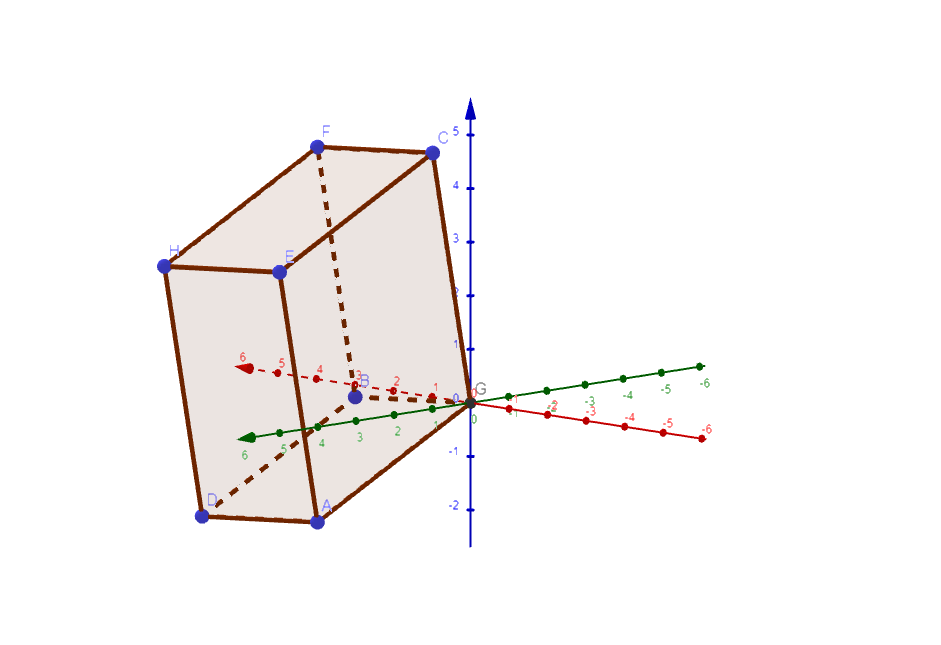
\includegraphics[width=\textwidth]{exercise-7-7.png}
		\caption{Exercise 7.7 - Fundamental domain of $L$}
	\end{figure}
	$\det (L) = \Vol (\mathcal{F})$
\end{exer}

\begin{exer}[7.43] $t = b_1 b_2 / \lVert b_1 \rVert^2$ and $b_2^* = b_2 - tb_1$ \\ $\Rightarrow b_2^* \cdot b_1 = b_1 (b_2 - tb_1) = b_1 b_2 - t \lVert b_1 \rVert^2 = b_1 b_2 - \frac{b_1 b_2}{\lVert b_1 \rVert^2} \cdot \lVert b_1 \rVert^2 = 0$ \\ Hence $b_2^* \perp b_1$ and $b_2^*$ is the projection of $b_2$ onto the orthogonal complement of $b_1$
\end{exer}

\begin{exer}[7.44]
	\begin{enumerate}
		\item [(a)] $\lVert a - tb \rVert^2 = (a - tb)^2 = a^2 - 2abt + t^2b^2 = \lVert a\rVert^2 + t^2 \lVert b\rVert^2 - 2abt \geq 0$ \\ $\Leftrightarrow a - tb = 0 \Rightarrow t = \frac{ab}{\lVert b \rVert^2}$
		\item [(b)] 0
		\item [(c)] $(a - tb)\cdot b = ab - t \lVert b \rVert^2 = ab - \frac{ab}{\lVert b \rVert^2} \cdot \lVert b \rVert^2 = 0$. \\ Therefore $a - tb$ is the projection of $a$ onto the orthogonal complement of $b$
	\end{enumerate}
\end{exer}

\begin{exer}[7.45]
	\begin{algorithm}
		\While{True}{
		\If{$\lVert v_2 \rVert < \lVert v_1 \rVert$}{swap $v_1$ and $v_2$}
		$m \gets \nint{v_1 \cdot v_2 / \lVert v_1 \rVert^2}$\;
		\If{$m = 0$}{return $(v_1, v_2)$}
		Replace $v_2$ with $v_2 - mv_1$
	}
	\TitleOfAlgo{Gauss's latice reduction algorithm}
	\end{algorithm}
	\begin{enumerate}
		\item [(a)] $v_1 = (14, -47)$, $v_2 = (-362, -131)$, 6 steps
		\item [(b)] $v_1 = (14, -47)$, $v_2 = (-362, -131)$, 6 steps
		\item [(c)] $v_1 = (147, 330)$, $v_2 = (690, -207)$, 7 steps
	\end{enumerate}
\end{exer}

\begin{exer}[7.46]
	\begin{enumerate}
		\item [(a)] $W^\perp$ is the orthogonal complement of $W$ in $V$ $\Rightarrow \vec{z} \in W^\perp$, $\vec{z}\cdot\vec{y} = 0, \forall \vec{y} \in W$ \\ With $\vec{z_1}, \vec{z_2} \in W^\perp \Rightarrow \vec{z_1}\cdot\vec{y} = \vec{z_2}\cdot\vec{y} = 0, \forall \vec{y} \in W$ \\ $\Rightarrow (\vec{z_1} + \vec{z_2})\cdot\vec{y} = 0 \Rightarrow \vec{z_1} + \vec{z_2} \in W^\perp$ \\ $\alpha\vec{z_1}\cdot\vec{y} = \alpha \cdot 0 = 0 \Rightarrow \alpha\vec{z_1} \in W^\perp, \forall \alpha \in \mathbb{R}$
		\item [(b)] We have 2 methods
		\begin{itemize}
			\item \textit{First method}: Show that $W \cup W^\perp = \{\vec{0}\}$. If $\vec{u}$ belongs to both $W$ and $W^\perp$, then $<u, u> = 0 \Rightarrow \vec{u} = \vec{0}$.
			
			Now denote $U = W + W^\perp$, we prove that $W = V$. We can choose an orthonormal basis in $U$ and extend it to orthonormal basis in $V$. Thus, if $U \neq V$, there is an element $\vec{e}$ in the basis of $V$ orthonormal to $U$. Since $U$ contains $W$, $e$ is orthonormal to $U \Rightarrow \vec{e} \in W^\perp$. The latter is a subspace of $W$, therefore $e$ is in $W$, which is contrary.
			\item \textit{Second method}: Let $\{e_1, e_2, \cdots, e_k\}$ be an orthonormal basis of the subspace $W$. For each $v \in V$, let $$P(v) = \sum_{j=1}^{k} <v, e_j> e_j$$ $$\Rightarrow (\forall v \in V): v = \underbrace{P(v)}_{\in W} + \underbrace{(v - P(v))}_{\in W^\perp}$$
			The fact that $v - P(v) \in W^\perp$ is: \\ if $j \in \{1, 2, \cdots, k\}$ then $$<v-P(v), e_j> = <v - \sum_{l=1}^{k}<v, e_l>e_l, e_j> = <v, e_j> - <v, e_j> = 0$$
			Since $\{e_1, \cdots, e_k\}$ is a basic of $W$, this prove that $v-P(v) \in W^\perp$
		\end{itemize}
		\item [(c)] $\lVert v \rVert^2 = <v, v> = (aw + bw')^2 = a^2w^2 + 2abww' + b^2w'^2 = a^2 \lVert w \rVert^2 + 0 + b^2 \lVert w' \rVert^2 = a^2 \lVert w \rVert^2 + b^2 \lvert w' \rVert^2$
	\end{enumerate}
\end{exer}

\end{document}